\chapter{Liouville's Theorem and Hamiltonian Flow}

This lecture is organized around a single question. In the first lecture we drew little reversible update rules with one arrow in and one arrow out, and we asked what the real classical-mechanical version of that idea ought to be. Liouville's theorem is the answer. But the theorem is not introduced as an isolated fact. We first step back, recall Hamilton's equations, reinterpret energy conservation geometrically, turn one phase point into a whole moving dust of phase points, and only then ask whether Hamiltonian flow compresses or not. In that order the theorem arrives with the right motivation: it becomes the continuous statement that Hamiltonian evolution loses no phase-space volume.

\section{Reversibility, Liouville, and a Historical Prelude}

The lecture opens with reversibility. We are promised a famous theorem, and the promise is precise: Liouville's theorem is the classical-mechanical analog of the earlier pictures in which a good law of physics had one arrow coming in and one arrow going out. In the discrete toy model that meant no ambiguity about the future and no ambiguity about the past. In classical mechanics the language will be different, but the underlying issue is the same. Do nearby states squeeze together and lose their individuality, or do they preserve their distinction?

Before any formulas are written, there is a deliberate historical pause. Hamilton, Lagrange, Jacobi, and Poisson did not know quantum mechanics, and yet they built one elegant formal structure after another. The lecture leans into that fact. The point is not biography for its own sake. The point is that Hamiltonian mechanics should be taken seriously as a formal reorganization of mechanics, one motivated by structure, analogy, and beauty as much as by any single concrete problem. Newton's equations were tied closely to celestial motion; the later formalism went further and tried to package mechanics into an axiomatic system.

That historical note matters here, because Liouville's theorem is a theorem about the formal structure of Hamiltonian motion. We are not yet trying to solve a particular problem. We are trying to understand what the Hamiltonian form of the laws guarantees.

\section{Hamilton's Equations and Conservation of the Hamiltonian}

We begin with canonical pairs
\begin{equation}
(q_i,p_i), \qquad i=1,\dots,n,
\end{equation}
one momentum for each coordinate and one coordinate for each momentum. The Hamiltonian is a function of all of them,
\begin{equation}
H(q,p),
\end{equation}
and it is the basic object out of which the equations of motion are packaged.

\begin{figure}[h]
\centering

\includegraphics[width=0.62\textwidth]{lecture_07_figure_02.png}
\caption{Generic Hamiltonian setup on the board: canonical variables, the Hamiltonian as a function of them, and the momentum-side Hamilton equation.}
\end{figure}

The lecture writes one Hamilton equation on the board and then supplies its partner:
\begin{align}
\dot p_i &= -\frac{\partial H}{\partial q_i}, \\
\dot q_i &= \frac{\partial H}{\partial p_i}.
\end{align}
These equations come in pairs, one pair for each index \(i\). The important point is that the right-hand side of any one equation may depend on all the canonical variables, since \(H\) itself is a function of all the \(q_j\) and \(p_j\).

It is also emphasized that at this stage the theory is axiomatic. There is no automatic assumption that \(p_i=m\dot q_i\). In simple systems the Hamiltonian often splits into kinetic plus potential terms, but once the formal structure is in hand we are free to study many other Hamiltonians as well.

Now let us derive conservation of the Hamiltonian in the standard way. The total time derivative is
\begin{equation}
\frac{dH}{dt}
=
\sum_i \frac{\partial H}{\partial p_i}\dot p_i
+
\sum_i \frac{\partial H}{\partial q_i}\dot q_i
+
\frac{\partial H}{\partial t}.
\end{equation}
The first two terms are present because the canonical variables move in time. The last term is present only if the Hamiltonian depends explicitly on time through changing external parameters.

Substituting Hamilton's equations gives
\begin{align}
\frac{dH}{dt}
&=
\sum_i \frac{\partial H}{\partial p_i}\left(-\frac{\partial H}{\partial q_i}\right)
+
\sum_i \frac{\partial H}{\partial q_i}\left(\frac{\partial H}{\partial p_i}\right)
+
\frac{\partial H}{\partial t} \\
&= \frac{\partial H}{\partial t}.
\end{align}
The summed terms cancel pairwise. Therefore, if the Hamiltonian has no explicit time dependence,
\begin{equation}
\frac{\partial H}{\partial t}=0
\qquad \Longrightarrow \qquad
\frac{dH}{dt}=0.
\end{equation}
That is the Hamiltonian form of energy conservation.

If \(\partial H/\partial t \neq 0\), the lecture interprets this in the usual way: some external system is changing in time and exchanging energy with the system under discussion. But for the central flow argument we keep the simpler time-translation-invariant case in view for the moment.

\section{Constant-Energy Surfaces in Phase Space}

Energy conservation immediately becomes a geometric statement. If \(H\) is constant along the motion, then the trajectory lies on a surface
\begin{equation}
H(q,p)=E,
\end{equation}
where \(E\) is fixed by the initial condition.

Phase space has \(2n\) dimensions when there are \(n\) coordinates and \(n\) conjugate momenta. A single equation such as \(H=E\) therefore defines a hypersurface of one lower dimension, namely a \((2n-1)\)-dimensional surface. The motion of the phase point stays on that surface.

The harmonic oscillator is the cleanest picture. In the lecture the normalization is loose, but the geometric content is unambiguous:
\begin{equation}
H_{\text{osc}} \propto p^2+q^2.
\end{equation}
Therefore the constant-energy curves satisfy
\begin{equation}
p^2+q^2=\text{constant},
\end{equation}
which are circles in the \(p\)-\(q\) plane.

\begin{figure}[h]
\centering
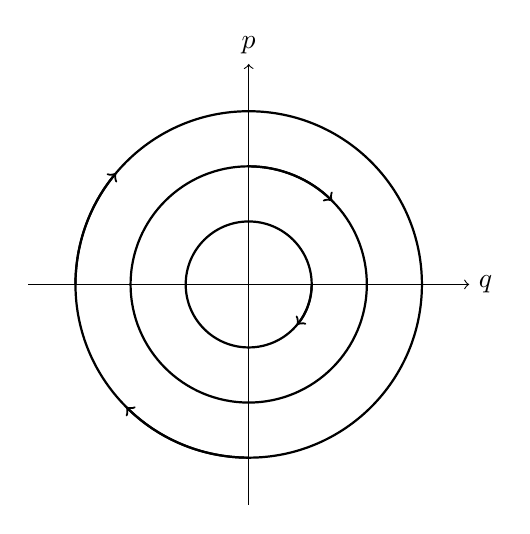
\begin{tikzpicture}[scale=1.0]
\draw[->] (-2.8,0) -- (2.8,0) node[right] {$q$};
\draw[->] (0,-2.8) -- (0,2.8) node[above] {$p$};

\draw[thick] (0,0) circle (0.8);
\draw[thick] (0,0) circle (1.5);
\draw[thick] (0,0) circle (2.2);

\draw[->,thick] (0.8,0) arc[start angle=0,end angle=-40,radius=0.8];
\draw[->,thick] (0,1.5) arc[start angle=90,end angle=45,radius=1.5];
\draw[->,thick] (-2.2,0) arc[start angle=180,end angle=140,radius=2.2];
\draw[->,thick] (0,-2.2) arc[start angle=-90,end angle=-135,radius=2.2];
\end{tikzpicture}
\caption{For the harmonic oscillator, the constant-energy curves are circles in the \(p\)-\(q\) plane, and the flow runs along them. In this special case the motion is a rigid rotation of the phase portrait.}
\end{figure}

\subsection{Question \& Answer}

\paragraph{Question.} How do the equations of motion differ from the constant-energy surface?

\paragraph{Answer.} They are not the same statement. The equations of motion tell us the velocity of the phase point at each point of phase space. The condition \(H=E\) tells us only the surface on which the motion is constrained to lie. Many different points lie on the same constant-energy surface. The equations of motion choose a definite tangent direction at each such point.

For the harmonic oscillator this distinction is especially transparent. The circles \(p^2+q^2=\text{constant}\) are the constant-energy curves. The Hamilton equations tell us how the point moves around each circle. One statement is about a locus in phase space; the other is about motion along that locus.

\section{From One Phase Point to a Fluid of Phase Points}

The next move is crucial. Instead of following one initial condition, we imagine all possible initial conditions at once. The phase plane is sprinkled with points. Every point is a possible state of the system, and every point moves according to the same Hamilton equations.

The lecture invites us to picture that sprinkling as an imaginary fluid, or if we prefer, as a dust so fine that it can be treated as continuous. This is only a visualization. The points do not represent physical particles of the original system. They represent states.

\begin{definition}
The \emph{phase-space velocity field} is the vector field whose components are the time derivatives of the canonical coordinates:
\begin{equation}
\mathbf V
=
(\dot q_1,\dots,\dot q_n,\dot p_1,\dots,\dot p_n).
\end{equation}
For a single canonical pair we may write
\begin{equation}
V_q=\dot q, \qquad V_p=\dot p.
\end{equation}
\end{definition}

Once the Hamiltonian is known, the field \(\mathbf V\) is known as a function of position in phase space. Wherever a phase point arrives, its instantaneous velocity is fixed by that point alone. In the harmonic oscillator this produces an especially simple flow: the whole pattern rotates as if it were mounted on a rigid carousel. Points nearer the origin move more slowly in magnitude, but they complete a revolution in the same period.

This is the shift from individual trajectories to flow. Liouville's theorem is not merely a statement about one orbit staying on one energy curve. It is a statement about what an extended patch of phase space does when every one of its points is evolved.

\subsection{Question \& Answer}

\paragraph{Question.} What is this fluid, exactly?

\paragraph{Answer.} It is not a new physical medium. It is a way of visualizing the collection of all possible states. If the language of fluid flow is helpful, we use it. If not, we can forget the fluid entirely and speak instead about a patch of phase space: take a region, evolve every point in it, and ask what happens to its volume. That is the content that matters.

The lecture is explicit on this point. The fluid picture is a convenient trick for the mind, not an extra ingredient in the mechanics.

\section{Compressibility, Divergence, and the Setup for Liouville}

Now we ask the real question: is this flow compressible?

In one dimension the answer is almost forced on us by intuition. If a one-dimensional fluid has velocity \(v(x)\), and if \(v\) increases as we move to the right, neighboring points spread apart. If \(v\) decreases, they bunch together. Thus the incompressible case is the case in which the velocity does not vary along the line:
\begin{equation}
\frac{dv}{dx}=0.
\end{equation}
Positive \(dv/dx\) means stretching; negative \(dv/dx\) means compression.

In more than one dimension the story changes slightly. A fluid may stretch in one direction and compress in another, preserving its total volume. That is why one must not demand that each individual derivative vanish. One demands only that the sum of the same-coordinate derivatives vanish.

\begin{definition}
For a vector field \(\mathbf V=(V_x,V_y,V_z)\), the \emph{divergence} is
\begin{equation}
\nabla\cdot \mathbf V
=
\frac{\partial V_x}{\partial x}
+
\frac{\partial V_y}{\partial y}
+
\frac{\partial V_z}{\partial z}.
\end{equation}
Incompressibility means
\begin{equation}
\nabla\cdot \mathbf V=0.
\end{equation}
In phase space the same idea applies, with one coordinate derivative for each canonical direction.
\end{definition}

For one canonical pair \((q,p)\), the phase-space divergence is
\begin{equation}
\frac{\partial V_p}{\partial p}+\frac{\partial V_q}{\partial q}.
\end{equation}
The first term measures bunching or stretching in the \(p\)-direction; the second does the same in the \(q\)-direction. Liouville's theorem will assert that their sum is zero.

At this point the lecture makes an important return to the first lecture. The continuous language of incompressible flow is the analog of the discrete reversible update rules. In the discrete picture a good law had one arrow in and one arrow out. In the continuous picture a good law has as much flow in as flow out.

\begin{figure}[h]
\centering
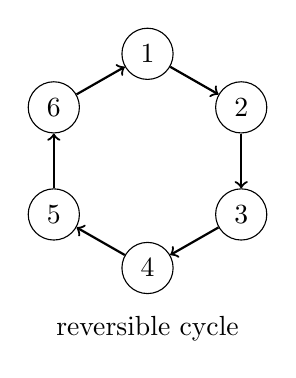
\begin{tikzpicture}[scale=0.85]
\foreach \x/\y/\name in {0/1.6/1,1.4/0.8/2,1.4/-0.8/3,0/-1.6/4,-1.4/-0.8/5,-1.4/0.8/6}
{
\node[circle,draw,minimum size=0.65cm] (\name) at (\x,\y) {\name};
}
\draw[->,thick] (1) -- (2);
\draw[->,thick] (2) -- (3);
\draw[->,thick] (3) -- (4);
\draw[->,thick] (4) -- (5);
\draw[->,thick] (5) -- (6);
\draw[->,thick] (6) -- (1);
\node at (0,-2.5) {reversible cycle};
\end{tikzpicture}
\hspace{1.2cm}
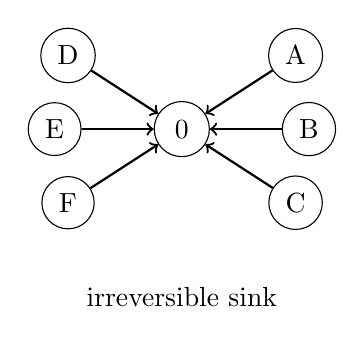
\begin{tikzpicture}[scale=0.85]
\node[circle,draw,minimum size=0.7cm] (c) at (0,0) {0};
\foreach \x/\y/\name in {1.7/1.1/A,1.9/0/B,1.7/-1.1/C,-1.7/1.1/D,-1.9/0/E,-1.7/-1.1/F}
{
\node[circle,draw,minimum size=0.65cm] (\name) at (\x,\y) {\name};
\draw[->,thick] (\name) -- (c);
}
\node at (0,-2.5) {irreversible sink};
\end{tikzpicture}
\caption{The lecture's earlier discrete pictures reappear here in continuous form. Reversible evolution corresponds to ``as much in as out''; irreversible evolution corresponds to a sink.}
\end{figure}

This is the correct setup for Liouville's theorem. We are no longer merely tracking a point on a constant-energy contour. We are examining the compressibility of the full Hamiltonian flow in phase space.

\section{Liouville's Theorem}

We now state the theorem in its natural language.

\begin{theorem}[Liouville's theorem]
For Hamiltonian motion, the phase-space velocity field is incompressible. Equivalently, the divergence of the phase-space flow vanishes, so any patch of phase space preserves its volume under time evolution.
\end{theorem}

\begin{proof}
Start with one canonical pair \((q,p)\). Define the phase-space velocity components by
\begin{equation}
V_p=\dot p, \qquad V_q=\dot q.
\end{equation}
The divergence is therefore
\begin{equation}
\frac{\partial V_p}{\partial p}+\frac{\partial V_q}{\partial q}.
\end{equation}
Now use Hamilton's equations:
\begin{equation}
V_p=-\frac{\partial H}{\partial q}, \qquad V_q=\frac{\partial H}{\partial p}.
\end{equation}
Substituting,
\begin{align}
\frac{\partial V_p}{\partial p}+\frac{\partial V_q}{\partial q}
&=
\frac{\partial}{\partial p}\!\left(-\frac{\partial H}{\partial q}\right)
+
\frac{\partial}{\partial q}\!\left(\frac{\partial H}{\partial p}\right) \\
&=
-\frac{\partial^2 H}{\partial p\,\partial q}
+
\frac{\partial^2 H}{\partial q\,\partial p}.
\end{align}
For an ordinary smooth function of two independent variables, the mixed partial derivatives are equal:
\begin{equation}
\frac{\partial^2 H}{\partial p\,\partial q}
=
\frac{\partial^2 H}{\partial q\,\partial p}.
\end{equation}
Hence
\begin{equation}
\frac{\partial V_p}{\partial p}+\frac{\partial V_q}{\partial q}=0.
\end{equation}

For many canonical pairs the same computation is repeated for each index:
\begin{equation}
\sum_i\left(
\frac{\partial \dot p_i}{\partial p_i}
+
\frac{\partial \dot q_i}{\partial q_i}
\right)=0.
\end{equation}
The cancellation happens pair by pair, one \(q_i\)--\(p_i\) pair at a time. Therefore the full Hamiltonian flow in phase space is incompressible.
\end{proof}

The lecture pauses over the equality of mixed partial derivatives and illustrates it by a small rectangle in the \(p\)-\(q\) plane. The finite-difference picture is elementary but useful: the second derivative is a difference of differences, and that combination is the same whichever order of differentiation one takes.

\begin{figure}[h]
\centering
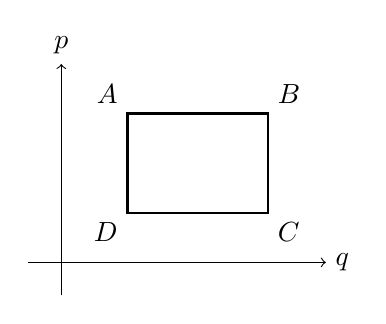
\begin{tikzpicture}[scale=1.05]
\draw[->] (-0.4,0) -- (3.2,0) node[right] {$q$};
\draw[->] (0,-0.4) -- (0,2.4) node[above] {$p$};
\draw[thick] (0.8,0.6) rectangle (2.5,1.8);
\node[above left] at (0.8,1.8) {$A$};
\node[above right] at (2.5,1.8) {$B$};
\node[below right] at (2.5,0.6) {$C$};
\node[below left] at (0.8,0.6) {$D$};
\end{tikzpicture}
\caption{The rectangle argument used in the lecture to motivate the equality of mixed partial derivatives. The mixed second derivative is the same difference-of-differences whichever order is taken.}
\end{figure}

What the theorem says geometrically is simple and powerful. If we take a patch of phase space and evolve every point in it, the patch may move, shear, stretch, and fold, but its phase-space volume does not change. Equivalently, if we stand at a fixed region and watch the flow pass through, as much comes in as goes out.

\subsection{Question \& Answer}

\paragraph{Question.} Why does Liouville's theorem survive even when the Hamiltonian depends explicitly on time, whereas conservation of energy did not?

\paragraph{Answer.} Conservation of energy concerns the time derivative of the Hamiltonian itself. That derivative contains the extra term \(\partial H/\partial t\), and it vanishes only when the Hamiltonian has no explicit time dependence. Liouville's theorem, by contrast, concerns derivatives of the velocity field with respect to the phase-space coordinates. In the one-pair proof the cancellation uses only
\[
\frac{\partial}{\partial p}\!\left(-\frac{\partial H}{\partial q}\right)
+
\frac{\partial}{\partial q}\!\left(\frac{\partial H}{\partial p}\right),
\]
and those terms still cancel even if \(H\) also depends on \(t\). The theorem is about the geometry of the Hamiltonian flow, not about the constancy of the Hamiltonian along the flow.

\section{Consequences, Counterexamples, and Outlook}

The theorem preserves volume, not rigidity. This distinction is essential. In the harmonic oscillator the motion is especially simple: a little patch in phase space rotates without changing either its area or its shape. But that is a special case. Liouville's theorem does \emph{not} say that general Hamiltonian evolution preserves shape, or angle, or circularity.

It does, however, say something strong. Distinct phase points do not coalesce into one. A region may become long and thin, but it does not collapse into a smaller-volume set. The lecture treats as an important informal consequence that a blob does not pinch off into disconnected pieces under the deterministic Hamiltonian flow. Each point has one and only one forward direction, fixed by the Hamiltonian, and that uniqueness prevents splitting at a point of contact.

A useful physical interpretation appears when ordinary space expands. If a gas occupies a larger region of \(q\)-space, then conservation of phase-space volume requires a compensating contraction in momentum space. That is the phase-space reason the momentum spread decreases and the gas cools. The lecture mentions the expanding universe only briefly; the central point is still the same: spreading in one set of directions must be compensated by compression in conjugate directions if the total phase-space volume is to remain fixed.

Now comes the lecture's sharp stress test.

\begin{figure}[h]
\centering

\includegraphics[width=0.58\textwidth]{lecture_07_figure_03.png}
\caption{The board at the beginning of the \(H=pq\) example: the Hamiltonian is written, and the first phase-space velocity relation is extracted from it.}
\end{figure}

Take the Hamiltonian
\begin{equation}
H=pq.
\end{equation}
This is not the usual quadratic oscillator Hamiltonian, but it is a perfectly legitimate Hamiltonian. The first velocity component is already visible on the board:
\begin{equation}
V_p=\dot p=-\frac{\partial H}{\partial q}.
\end{equation}
Carrying out the derivative gives
\begin{equation}
\dot p=-p.
\end{equation}
Likewise
\begin{equation}
\dot q=\frac{\partial H}{\partial p}=q.
\end{equation}
So the motion compresses exponentially in the \(p\)-direction and expands exponentially in the \(q\)-direction. A small square patch becomes a long thin strip. Yet the divergence is still zero:
\begin{equation}
\frac{\partial V_p}{\partial p}+\frac{\partial V_q}{\partial q}
=
(-1)+(1)=0.
\end{equation}
Area is preserved even though shape changes violently.

\begin{remark}
The product \(pq\) has the units of action, and a phase-space area element has the units of action as well. But Liouville's theorem is not the conservation of the action. What is conserved here is volume in phase space.
\end{remark}

\begin{figure}[h]
\centering
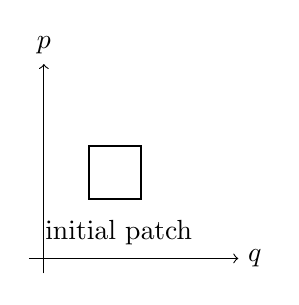
\begin{tikzpicture}[scale=0.95]
\draw[->] (-0.2,0) -- (2.6,0) node[right] {$q$};
\draw[->] (0,-0.2) -- (0,2.6) node[above] {$p$};
\draw[thick] (0.6,0.8) rectangle (1.3,1.5);
\node at (1.0,0.35) {initial patch};
\end{tikzpicture}
\hspace{1.0cm}
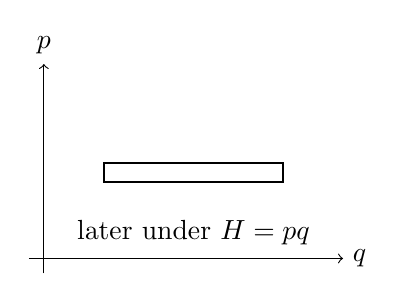
\begin{tikzpicture}[scale=0.95]
\draw[->] (-0.2,0) -- (4.0,0) node[right] {$q$};
\draw[->] (0,-0.2) -- (0,2.6) node[above] {$p$};
\draw[thick] (0.8,1.02) rectangle (3.2,1.28);
\node at (2.0,0.35) {later under \(H=pq\)};
\end{tikzpicture}

\vspace{0.8cm}

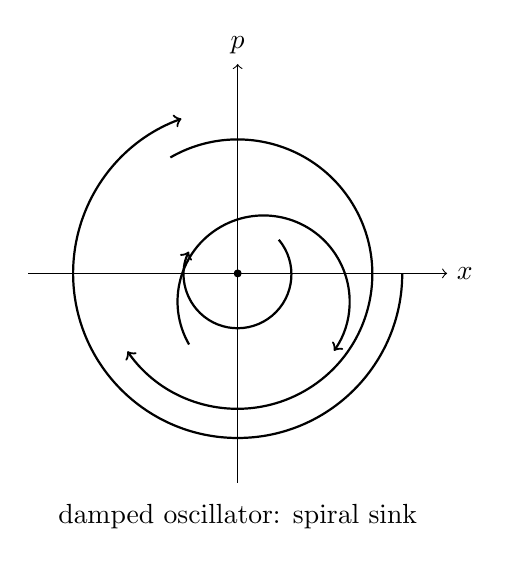
\begin{tikzpicture}[scale=0.95]
\draw[->] (-2.8,0) -- (2.8,0) node[right] {$x$};
\draw[->] (0,-2.8) -- (0,2.8) node[above] {$p$};
\draw[->,thick] (2.2,0) arc[start angle=0,end angle=-250,radius=2.2];
\draw[->,thick] (-0.9,1.55) arc[start angle=120,end angle=-145,radius=1.8];
\draw[->,thick] (-0.65,-0.95) arc[start angle=210,end angle=-35,radius=1.15];
\draw[->,thick] (0.55,0.45) arc[start angle=40,end angle=-205,radius=0.72];
\filldraw (0,0) circle (1.3pt);
\node at (0,-3.25) {damped oscillator: spiral sink};
\end{tikzpicture}
\caption{Top: the \(H=pq\) flow stretches a patch in the \(q\)-direction and squeezes it in the \(p\)-direction, preserving area but not shape. Bottom: the damped oscillator contracts toward the origin and therefore does \emph{not} satisfy Liouville's theorem.}
\end{figure}

To see what fails when the motion is not Hamiltonian, consider the damped harmonic oscillator,
\begin{equation}
m\ddot x=-kx-c\dot x.
\end{equation}
If we define \(p=m\dot x\), then the phase-space equations are
\begin{equation}
\dot x=\frac{p}{m}, \qquad \dot p=-kx-\frac{c}{m}p.
\end{equation}
The divergence is
\begin{equation}
\frac{\partial \dot x}{\partial x}+\frac{\partial \dot p}{\partial p}
=
0-\frac{c}{m}<0.
\end{equation}
Now the flow has negative divergence. The phase portrait spirals inward. A patch of phase space shrinks toward the origin. This is the lecture's continuous analog of a sink in the old discrete diagrams. Such a system is not generated by a Hamiltonian; the viscous term does not come from a potential, and within this reduced description information is effectively lost.

\subsection{Question \& Answer}

\paragraph{Question.} Can divergence vanish without a Hamiltonian?

\paragraph{Answer.} Yes. Hamiltonian flow is sufficient for zero divergence, but it is not necessary. The lecture gives the example of an ordinary incompressible fluid in three spatial dimensions. Its velocity field can have zero divergence, but it does not come from a Hamiltonian of the sort used here, since Hamiltonian phase space is even-dimensional. Thus the implication is one-way:
\begin{equation}
\text{Hamiltonian flow} \Longrightarrow \text{incompressible phase-space flow},
\end{equation}
but not conversely.

There is one last bridge. If \(F(q,p)\) is any function on phase space, then its time derivative is
\begin{equation}
\frac{dF}{dt}
=
\sum_i\left(
\frac{\partial F}{\partial q_i}\dot q_i
+
\frac{\partial F}{\partial p_i}\dot p_i
\right)
=
\sum_i\left(
\frac{\partial F}{\partial q_i}\frac{\partial H}{\partial p_i}
-
\frac{\partial F}{\partial p_i}\frac{\partial H}{\partial q_i}
\right).
\end{equation}
This is the form that Poisson packages into the bracket
\begin{equation}
\frac{dF}{dt}=\{F,H\}.
\end{equation}
The lecture stops there. The point is not yet to develop Poisson brackets in full, but to show that Hamiltonian mechanics can be repackaged once again into a still more condensed language.

\section{Summary}

Liouville's theorem is the continuous classical statement that Hamiltonian evolution does not squeeze phase-space volume away. We reached it in the same order as the lecture: Hamilton's equations, conservation of the Hamiltonian, constant-energy surfaces, a fluid picture in phase space, the notion of divergence, and then the cancellation of mixed partial derivatives. The payoff is geometric and conceptual at once. Volume in phase space is preserved; shape need not be. The example \(H=pq\) shows violent stretching and squeezing with zero divergence, while the damped oscillator shows what a true sink looks like when Hamiltonian structure is abandoned. That is why Liouville's theorem is the right classical analog of reversibility: it is the statement that Hamiltonian flow has as much going out as coming in.